\documentclass[12pt,a4paper]{article}

\usepackage{amsmath}
\usepackage{amssymb}
\usepackage{amsthm}
%\pagestyle{empty}
\usepackage[margin=1in]{geometry}
\usepackage{hyperref}
\usepackage[utf8]{inputenc}
\usepackage[IL2]{fontenc}
\usepackage[czech]{babel}
\usepackage{graphicx}

%\def\vysl#1{}
\newcommand{\R}{\mathbb R}
\DeclareMathOperator{\tg}{tg}

\newtheorem*{veta}{Věta}

\theoremstyle{definition}

\newtheorem{uloha}{Úloha}

\newenvironment{res}{\proof}{\endproof}

\begin{document}
\renewcommand*{\proofname}{Řešení}

\section*{Nějaká další fakta}

\begin{veta}[\uv{O třech limitách}, též \uv{O dvou policajtech}]
Nechť tři funkce $f$, $g$, $h$ splňují $f(x) \leq g(x) \leq h(x)$ pro všechna $x$ z nějakého prstencového okolí bodu $c \in \R^*$. Dále nechť $f$ a $h$ mají v $c$ vlastní limitu $A$. Pak i $g$ má v $c$ limitu $A$.
\end{veta}

Z aplikací a obrázků bude snad dobře \uv{vidět}, proč tato věta platí; prostřední funkce je \uv{sevřena} těmi krajními, takže nemá jinou možnost, než mít v $c$ tutéž limitu:

\begin{uloha}
Dokažte, že
\[ \lim_{x \to \infty} \frac{x}{x + \sin x} = 1. \]
\end{uloha}
\begin{res}
Pro všechna reálná $x$ platí $-1 \leq \sin x \leq 1$, proto pro $x > 1$ platí
\[ \frac{x}{x + 1} \leq \frac{x}{x + \sin x} \leq \frac{x}{x - 1}. \]
Jelikož
\[ \lim_{x \to \infty} \frac{x}{x + 1} = \lim_{x \to \infty} \frac{x}{x - 1} = 1, \]
je také
\[ \lim_{x \to \infty} \frac{x}{x + \sin x} = 1. \]
\[ 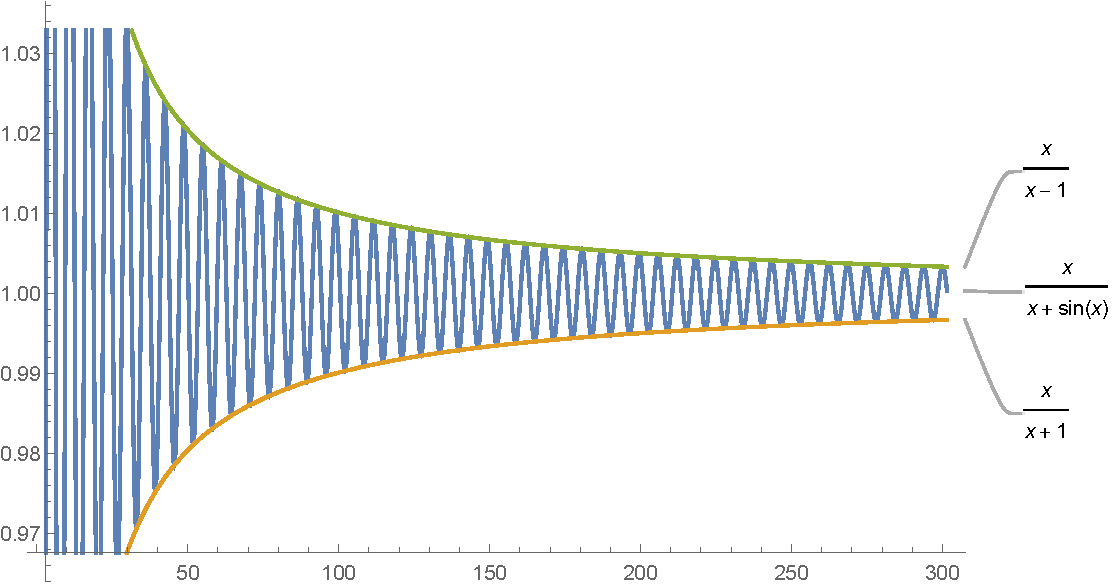
\includegraphics[scale=.65]{grafy_3/infty.pdf} \]
\end{res}


\begin{uloha}
Dokažte, že
\[ \lim_{x \to 0} x \sin \tfrac 1x = 0. \]
\end{uloha}
\begin{res}
Pro všechna $x \neq 0$ platí $-1 \leq \sin \frac 1x \leq 1$, proto pro $x \neq 0$ rovněž platí
\[ -|x| \leq x \sin \tfrac 1x \leq |x|. \]
Jelikož
\[ \lim_{x \to 0} (-|x|) = \lim_{x \to 0} |x| = 0, \]
je také
\[ \lim_{x \to 0} x \sin \tfrac 1x = 0. \]
\[ 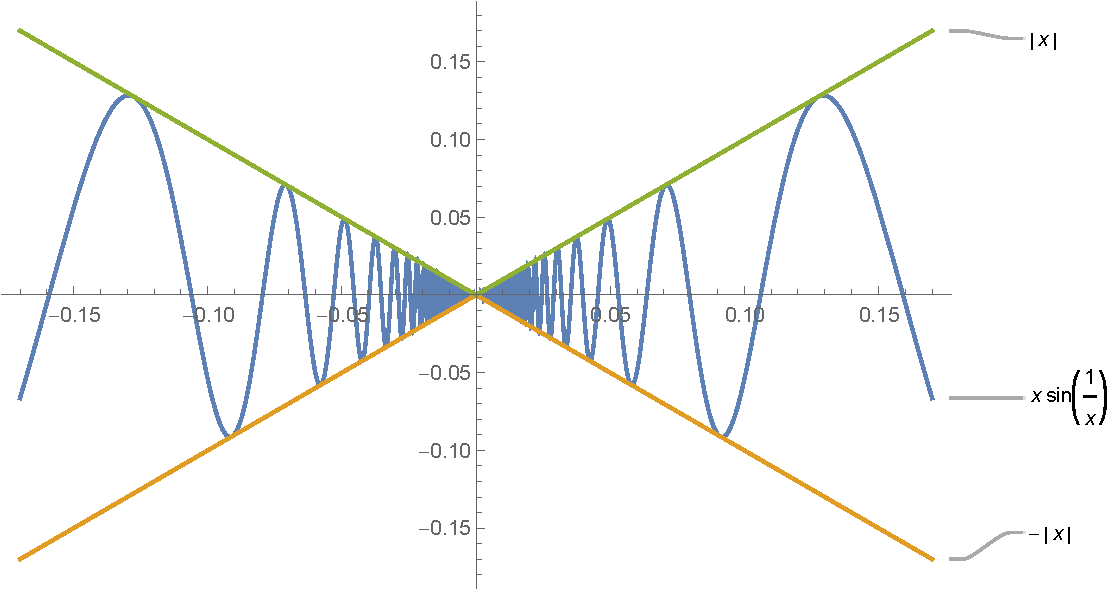
\includegraphics[scale=.65]{grafy_3/nula.pdf} \]
\end{res}

Konečně se dostáváme k naší oblíbené limitě!

\begin{uloha}
Dokažte, že
\[ \lim_{x \to 0} \frac{\sin x}{x} = 1. \]
\end{uloha}
\begin{res}
Z hodiny víme, že $\sin x \leq x$ pro $x \geq 0$, což se nahlédne z definice sinu pomocí jednotkové kružnice:
\[ 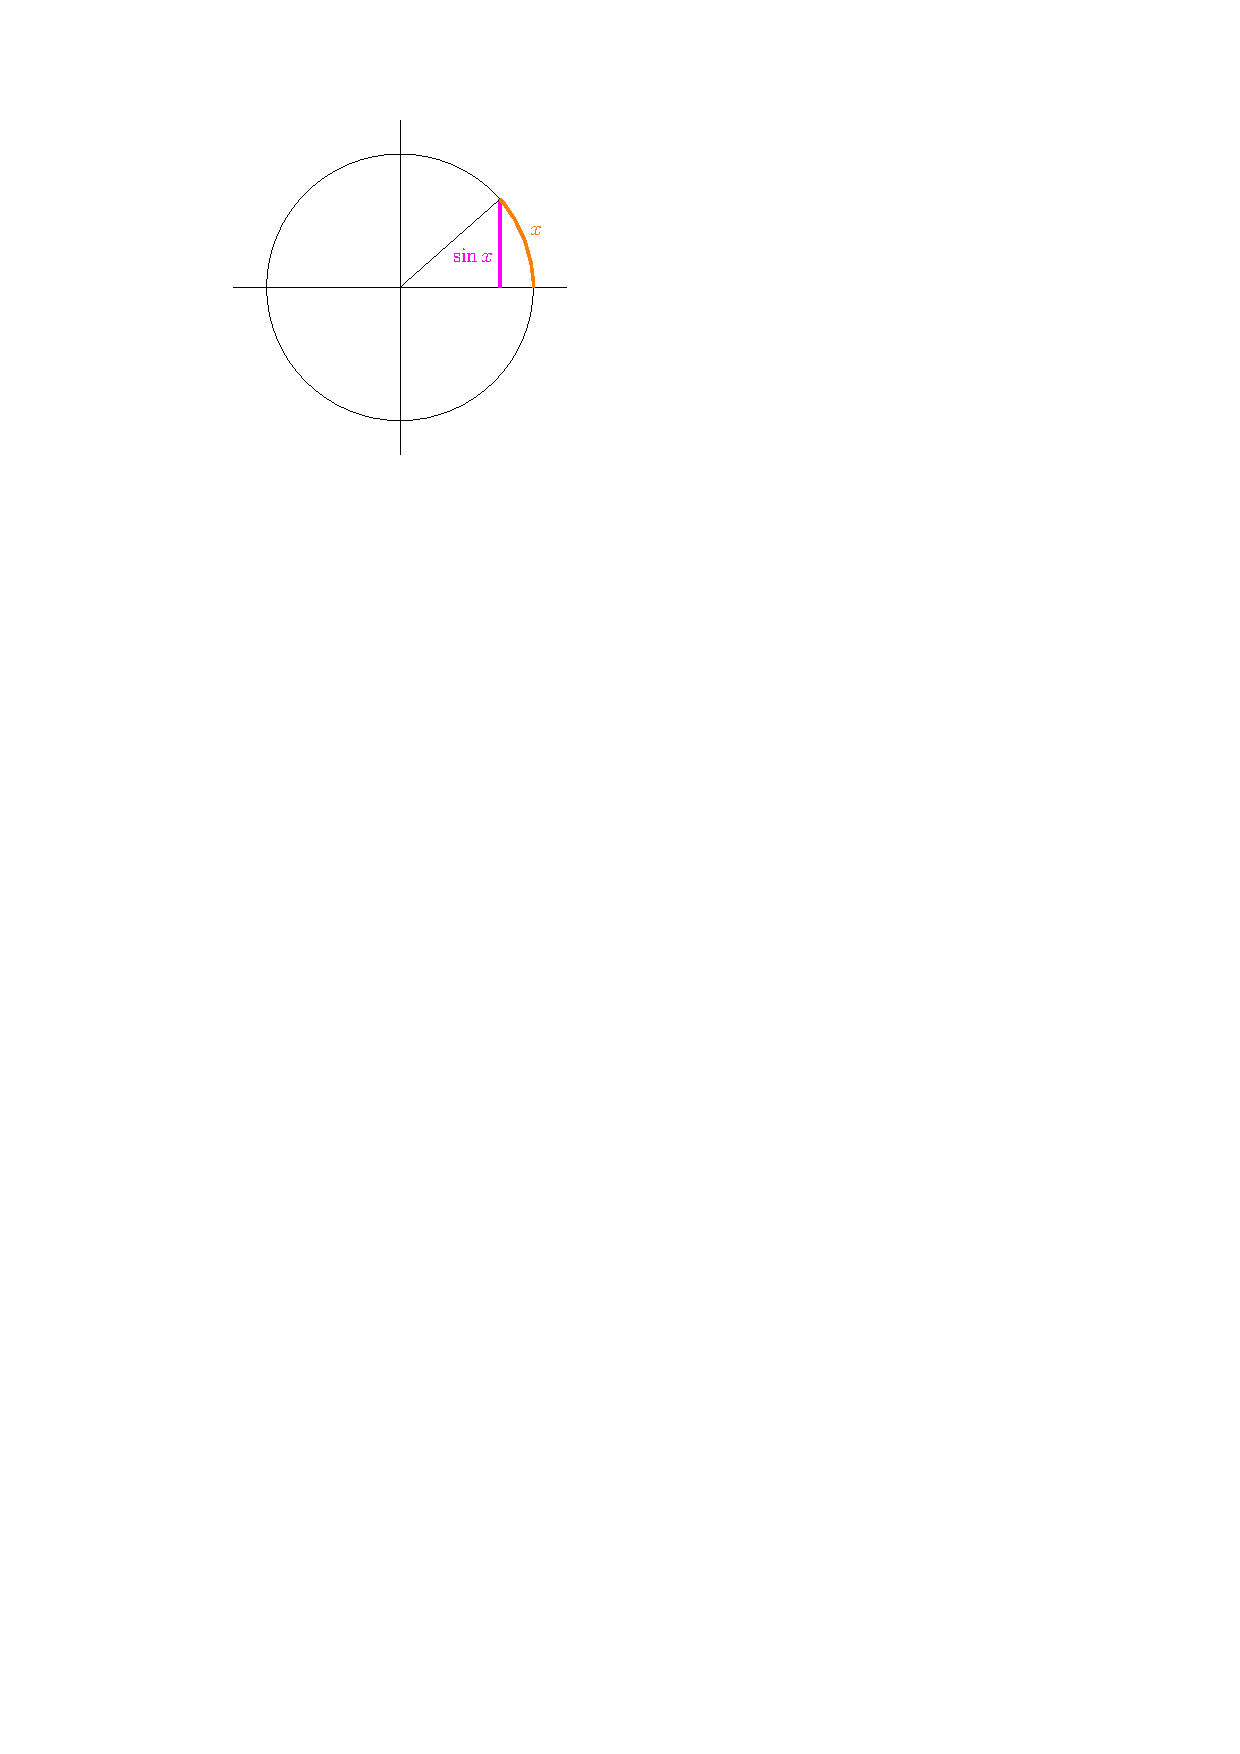
\includegraphics{grafy_3/kruz_sin.pdf} \]
Pro $x \leq 0$ naopak dostaneme $\sin x \geq x$, ovšem obě tyto nerovnosti přejdou po podělení $x$ ve
\[ \frac{\sin x}{x} \leq 1 \]
pro $x \neq 0$ (v té záporné se otočilo znaménko).

V druhém kroce nahlédneme, že pro $x \in (0; \pi/2)$ ještě platí $\tg x \geq x$; opět budeme postupovat přes jednotkovou kružnici, ale teď to bude lehce zajímavější:
\[ 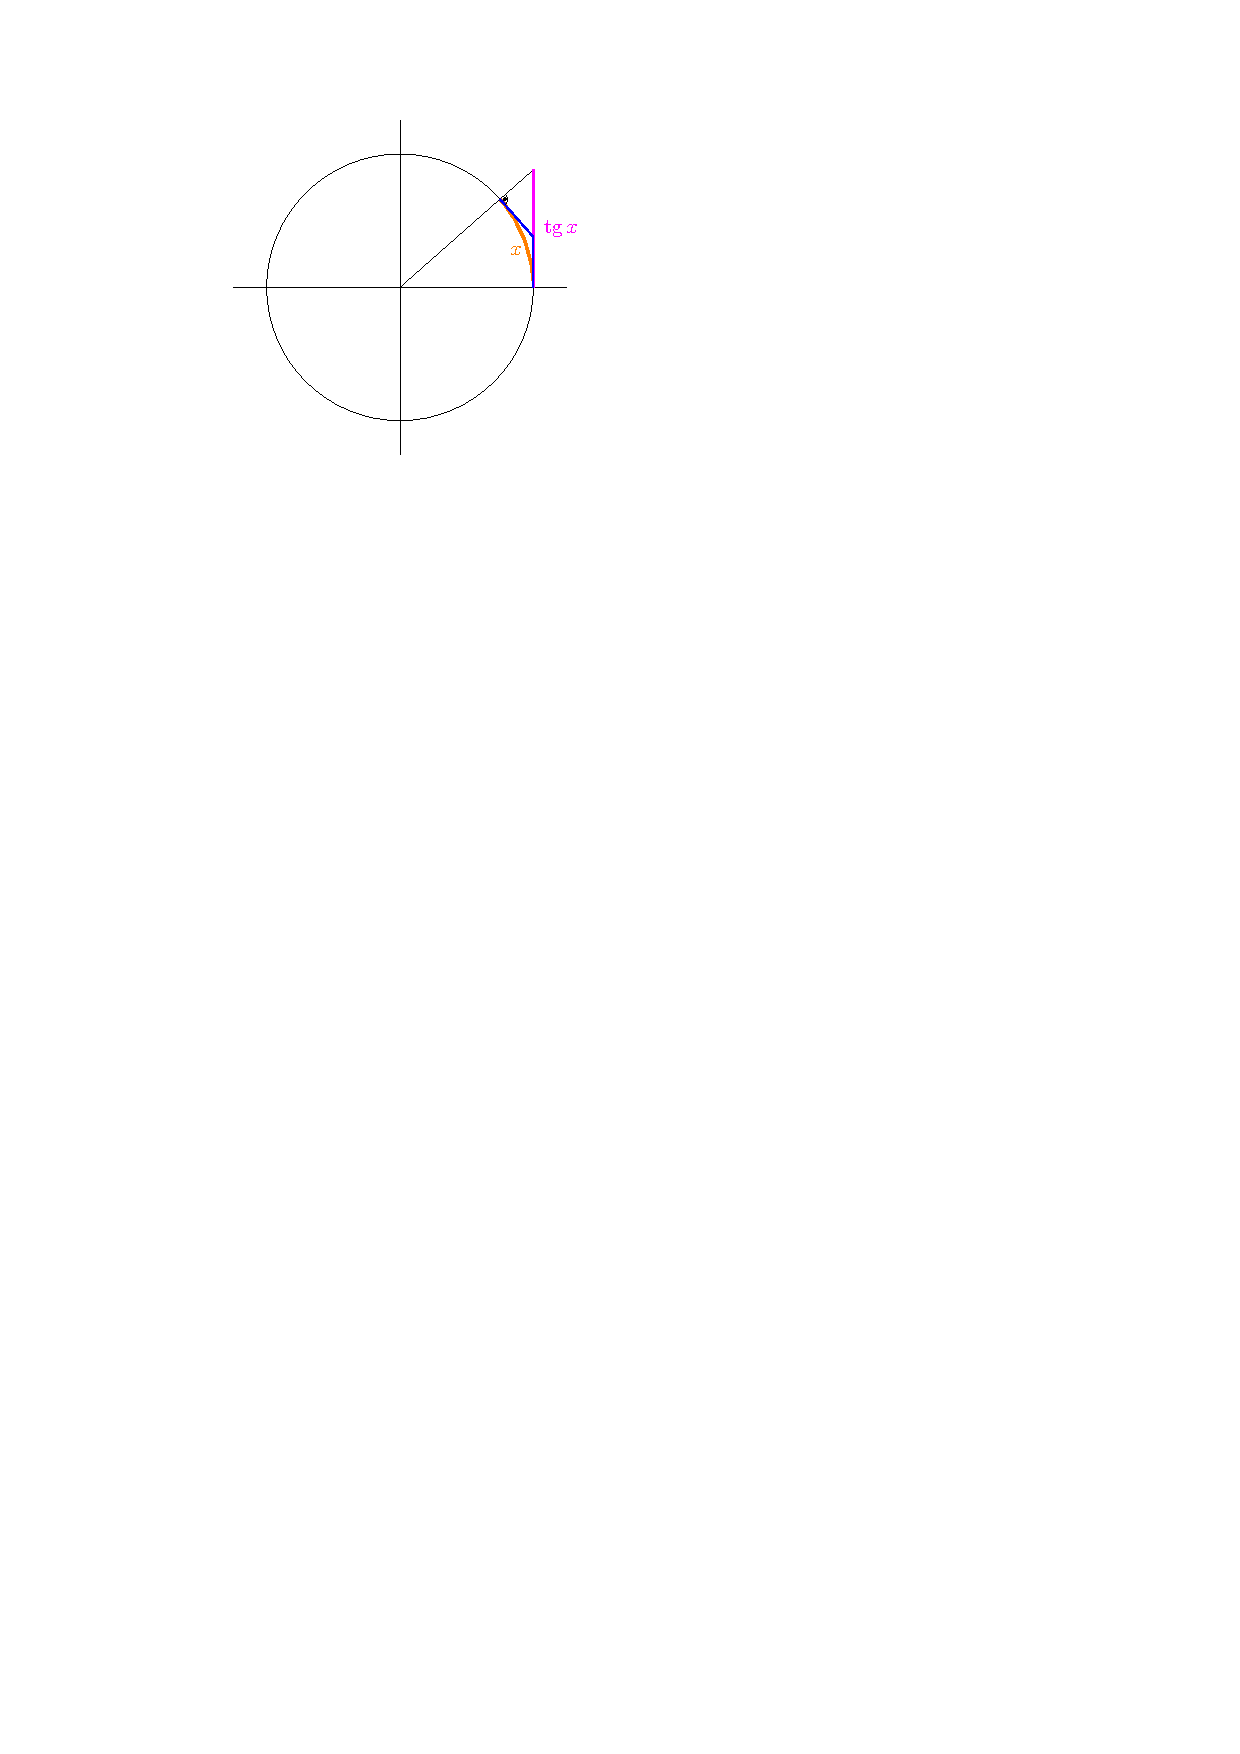
\includegraphics{grafy_3/kruz_tg2.pdf} \]
Délka oblouku, což je $x$, je menší než délka modré lomené čáry (která je tečná k oblouku v~krajních bodech). Úsečka odpovídající $\tg x$ je ovšem ještě delší -- \uv{horní} usek je přepona v pravoúhlém trojúhelníku, zatímco modrý segment je pouze odvěsnou.

Pro $x \in (\pi/2; 0)$ máme opět opačnou nerovnost $\tg x \leq x$; každopádně po vydělení $x$ získáváme
\[ \frac{\tg x}{x} \geq 1 \]
což si po přenásobení $\cos x$ (který je kladný na intervalu $(-\pi/2, \pi/2)$) ještě změníme na
\[ \frac{\sin x}{x} \geq \cos x \]
pro $x \in (-\pi/2, \pi/2)$, $x \neq 0$ (což se dá říct i jako $x \in P(0; \pi/2)$).

Vidíme tedy, že pro $x \in P(0; \pi/2)$ máme
\[ \cos x \leq \frac{\sin x}{x} \leq 1 \]
a jelikož
\[ \lim_{x \to 0} \cos x = \lim_{x \to 0} 1 = 1, \]
je také
\[ \lim_{x \to 0} \frac{\sin x}{x} = 1. \]
\[ 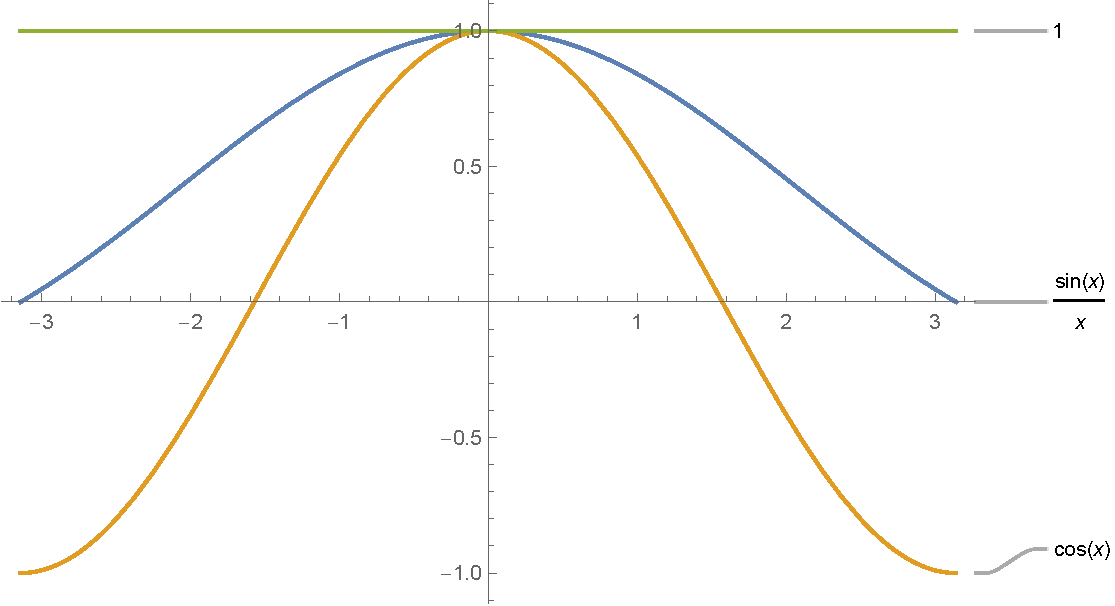
\includegraphics[scale=.65]{grafy_3/sinx.pdf} \]
\end{res}
\end{document}